\casesection{Uniform sediment with variable d50 (sed-mor)}
\label{case:e02-f22-c06}
%------------------------------------------------------------------------------
\paragraph*{Purpose}

The purpose of this validation case is to examine the performance of D-Flow FM-sed-mor in simulating uniform sediment. A straight channel flow simulations with minor longitudinal slope and trench in middle of the channel has been prescribed. The test case number is e02-f22-c06.
\paragraph*{Linked claims}
%\begin{itemize}
%	\item
The variable sediment grain size in module performs well, according to the comparison executed between two simulations (with structured and unstructured grid) of the test case.
%\end{itemize} 
\paragraph*{Approach}
two simulations have been prepared
%\begin{enumerate}
%	\item 
and all the input is specified using D-Flow flexible mesh (FM)-sed-mor module.
%\end{enumerate}

\paragraph*{Model Description}
In this test case  we use a network of straight channel. A straight channel flows with a constant roughness factor under equilibrium flow conditions. A discharge $Q$ varies between 0.0-1.0 m$^3$/s is prescribed as an upstream boundary condition. The longitudinal bottom slope $i_b$ is prescribed to be $0.012$ (see figure \ref{fig:C06}). The length of the channel is 10 km, while the width of the channel is 100 m . The chezy friction coefficient $C$ is set to 65 $m^{1/2}/s$. The downstream boundary condition is water level set to 0.00 m.

In this test-case:
\begin{itemize}
	\item[$\bullet$] variable sediment grain size D{50} is used. d50 file is generated with basically two d50 sizes as shown in the longitudinal section in figure \ref{fig:ATH}.
\end{itemize}
The default parameters in the morphological setup are mainly used.Nevertheless, in the following part  important related setup of morphology and sediment files used are described as follows:
\begin{itemize}
	\item[$\bullet$] Sediment file $<*.sed>$:
\end{itemize}

\begin{verbatim}
[Sediment]
SedTyp           = Sand       # Must be "sand", "mud" or "bedload"
SedDia           = #test.d50#   # [m] Median sediment diameter (D50)
\end{verbatim}
$SedTyp$ is sand,
Sediment transport equation is the default formula (Van Rijn (1993)) and
sediment grain size ($D_{50}$) is variable.
\begin{itemize}
	\item[$\bullet$] Morphology file $<*.mor>$:
\end{itemize}
The morphological update $ MorUpd$ and bed composition update  $CmpUpd$ are switched on. $MorFac$ is equal to 15 and the spin-up interval from the start time until the start of morphological changes $MorStt$ is 0.0 minutes.

Two models are set up one with structured grid and the second model with unstructured grid. The results of the bed change along channel centerline are compared as shown in figure \ref{fig:5.5d}  and  \ref{fig:18d}.
\begin{figure}[h!]
	\begin{center}
		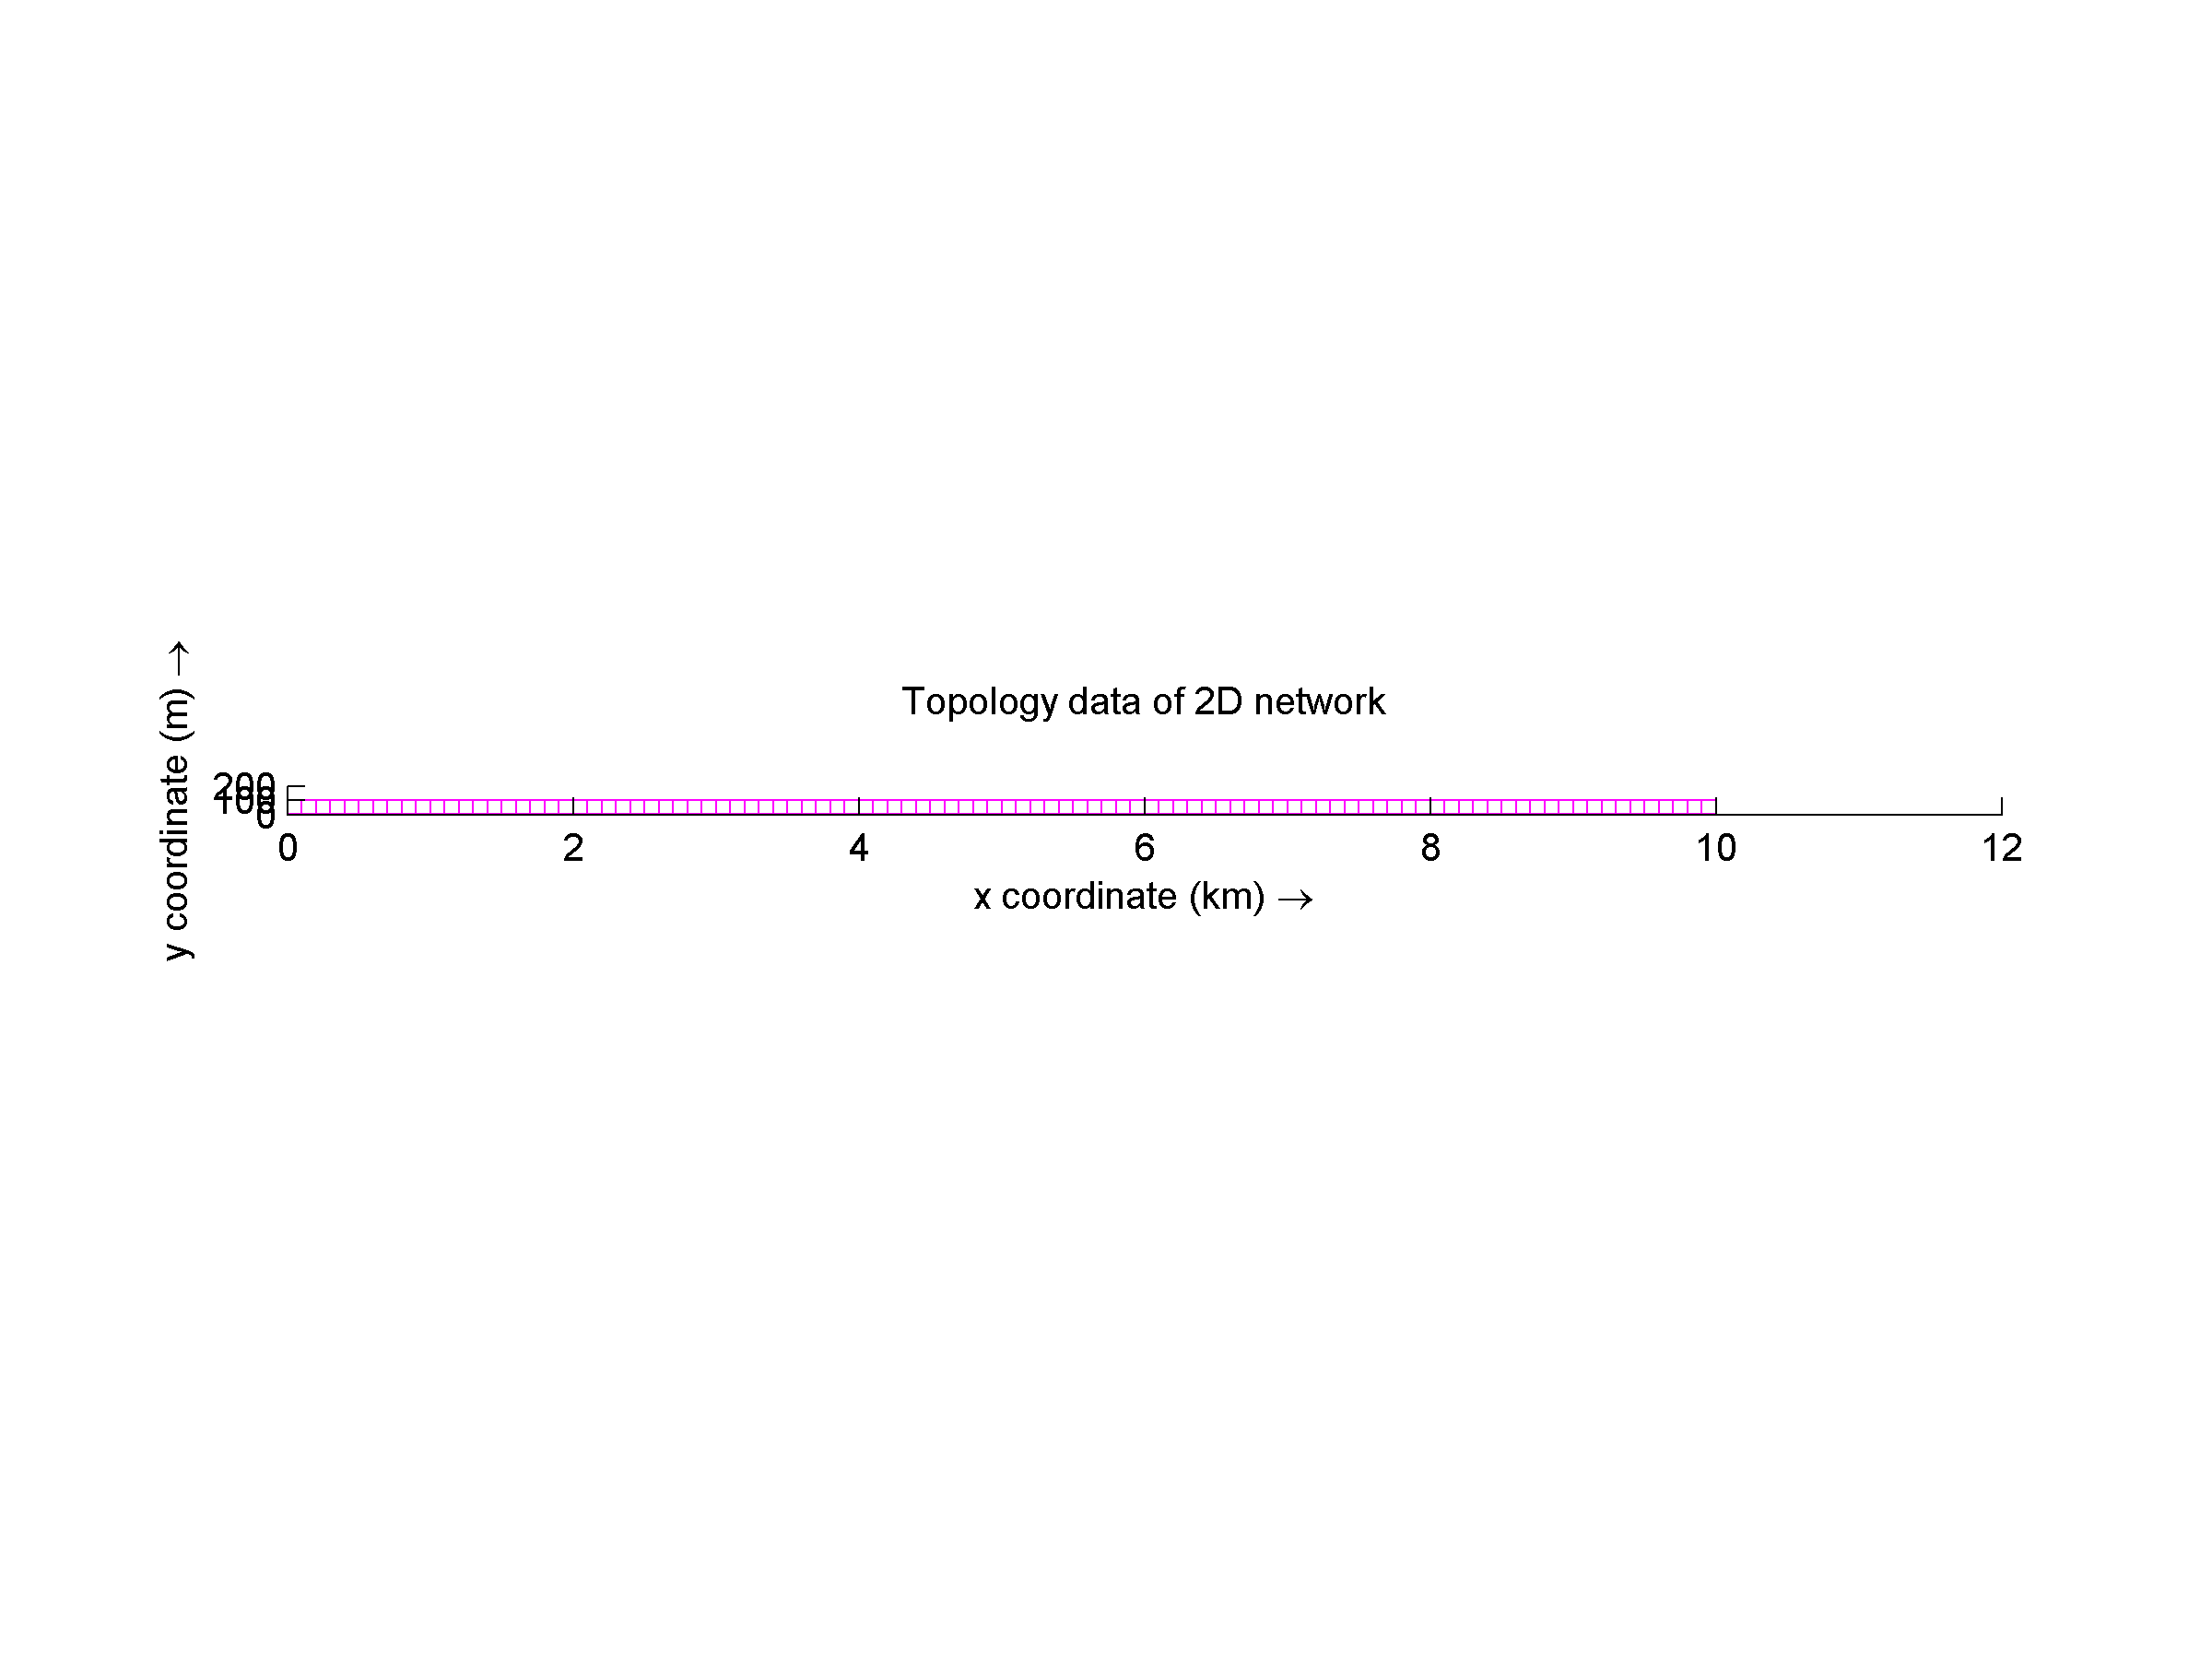
\includegraphics[width=0.7\columnwidth] {figures/c06net.png}
	\end{center}\caption{c06 net}
	\label{fig:C06}
\end{figure}

\begin{figure}[h!]
	\begin{center}
		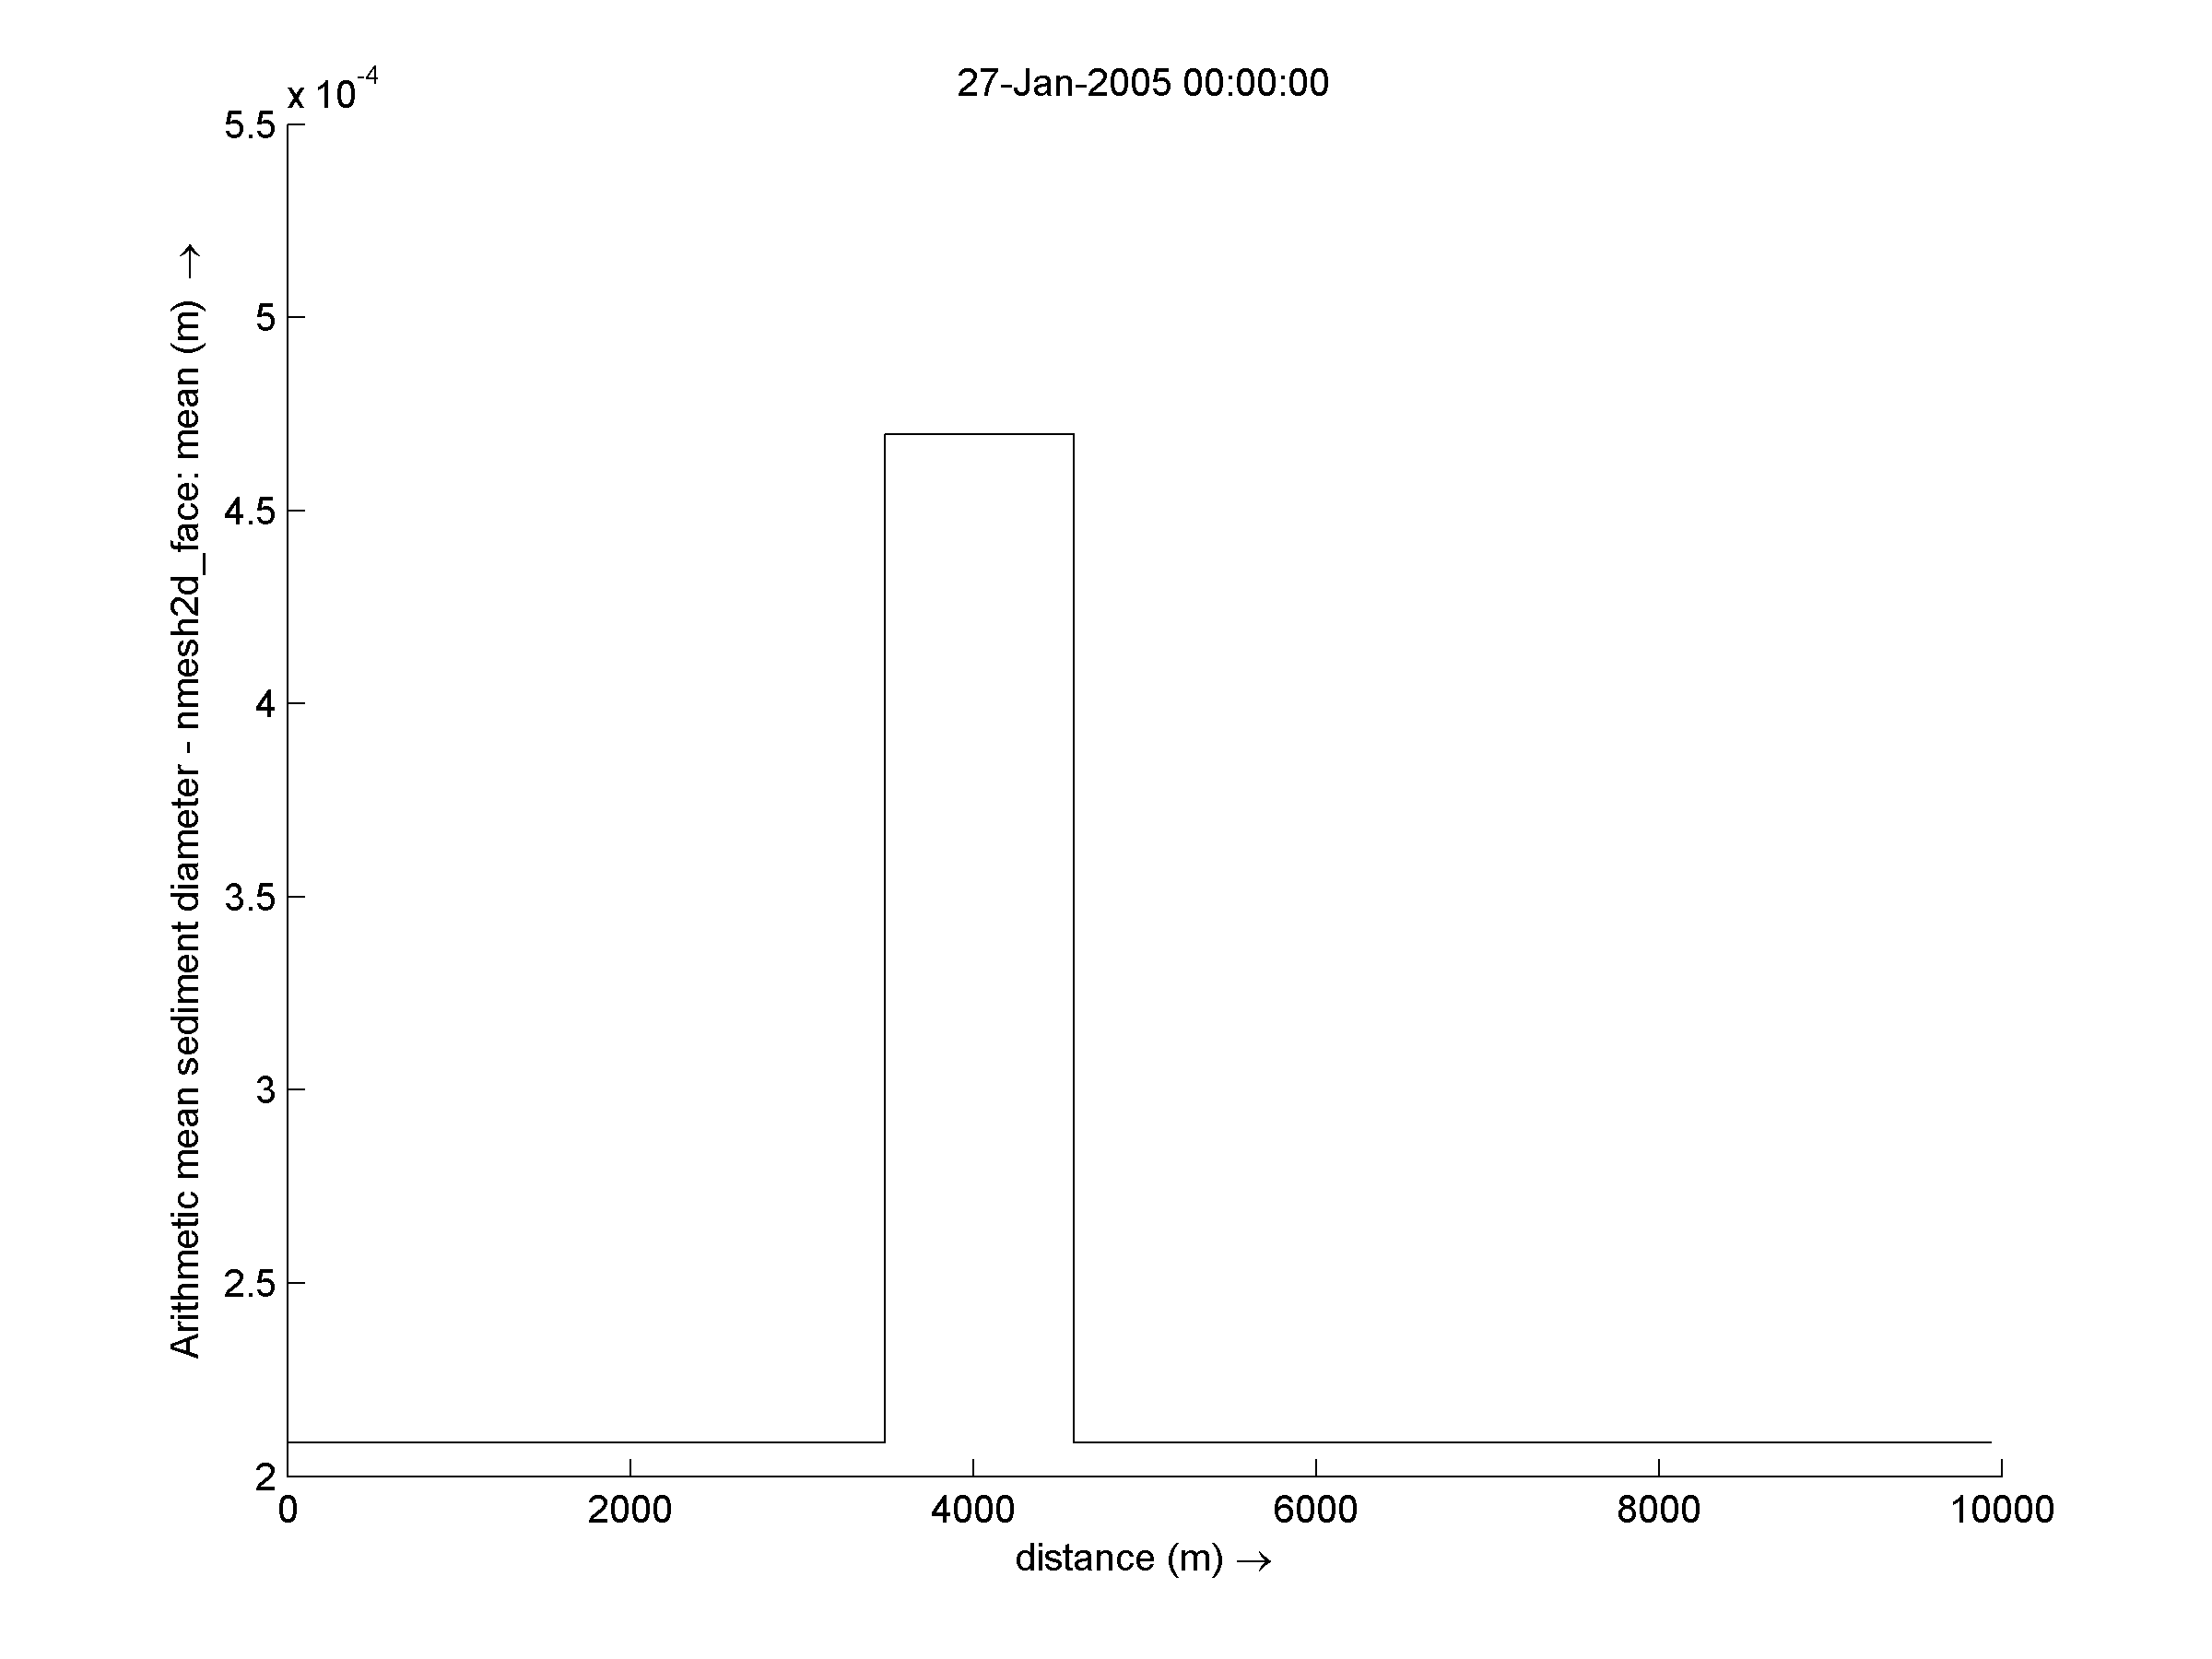
\includegraphics[width=0.7\columnwidth] {figures/ATH-DIAMETER.png}
	\end{center}\caption{C06 the grain size distribution along the channel centerline}
	\label{fig:ATH}
\end{figure}

\begin{figure}[h!]
	\begin{center}
		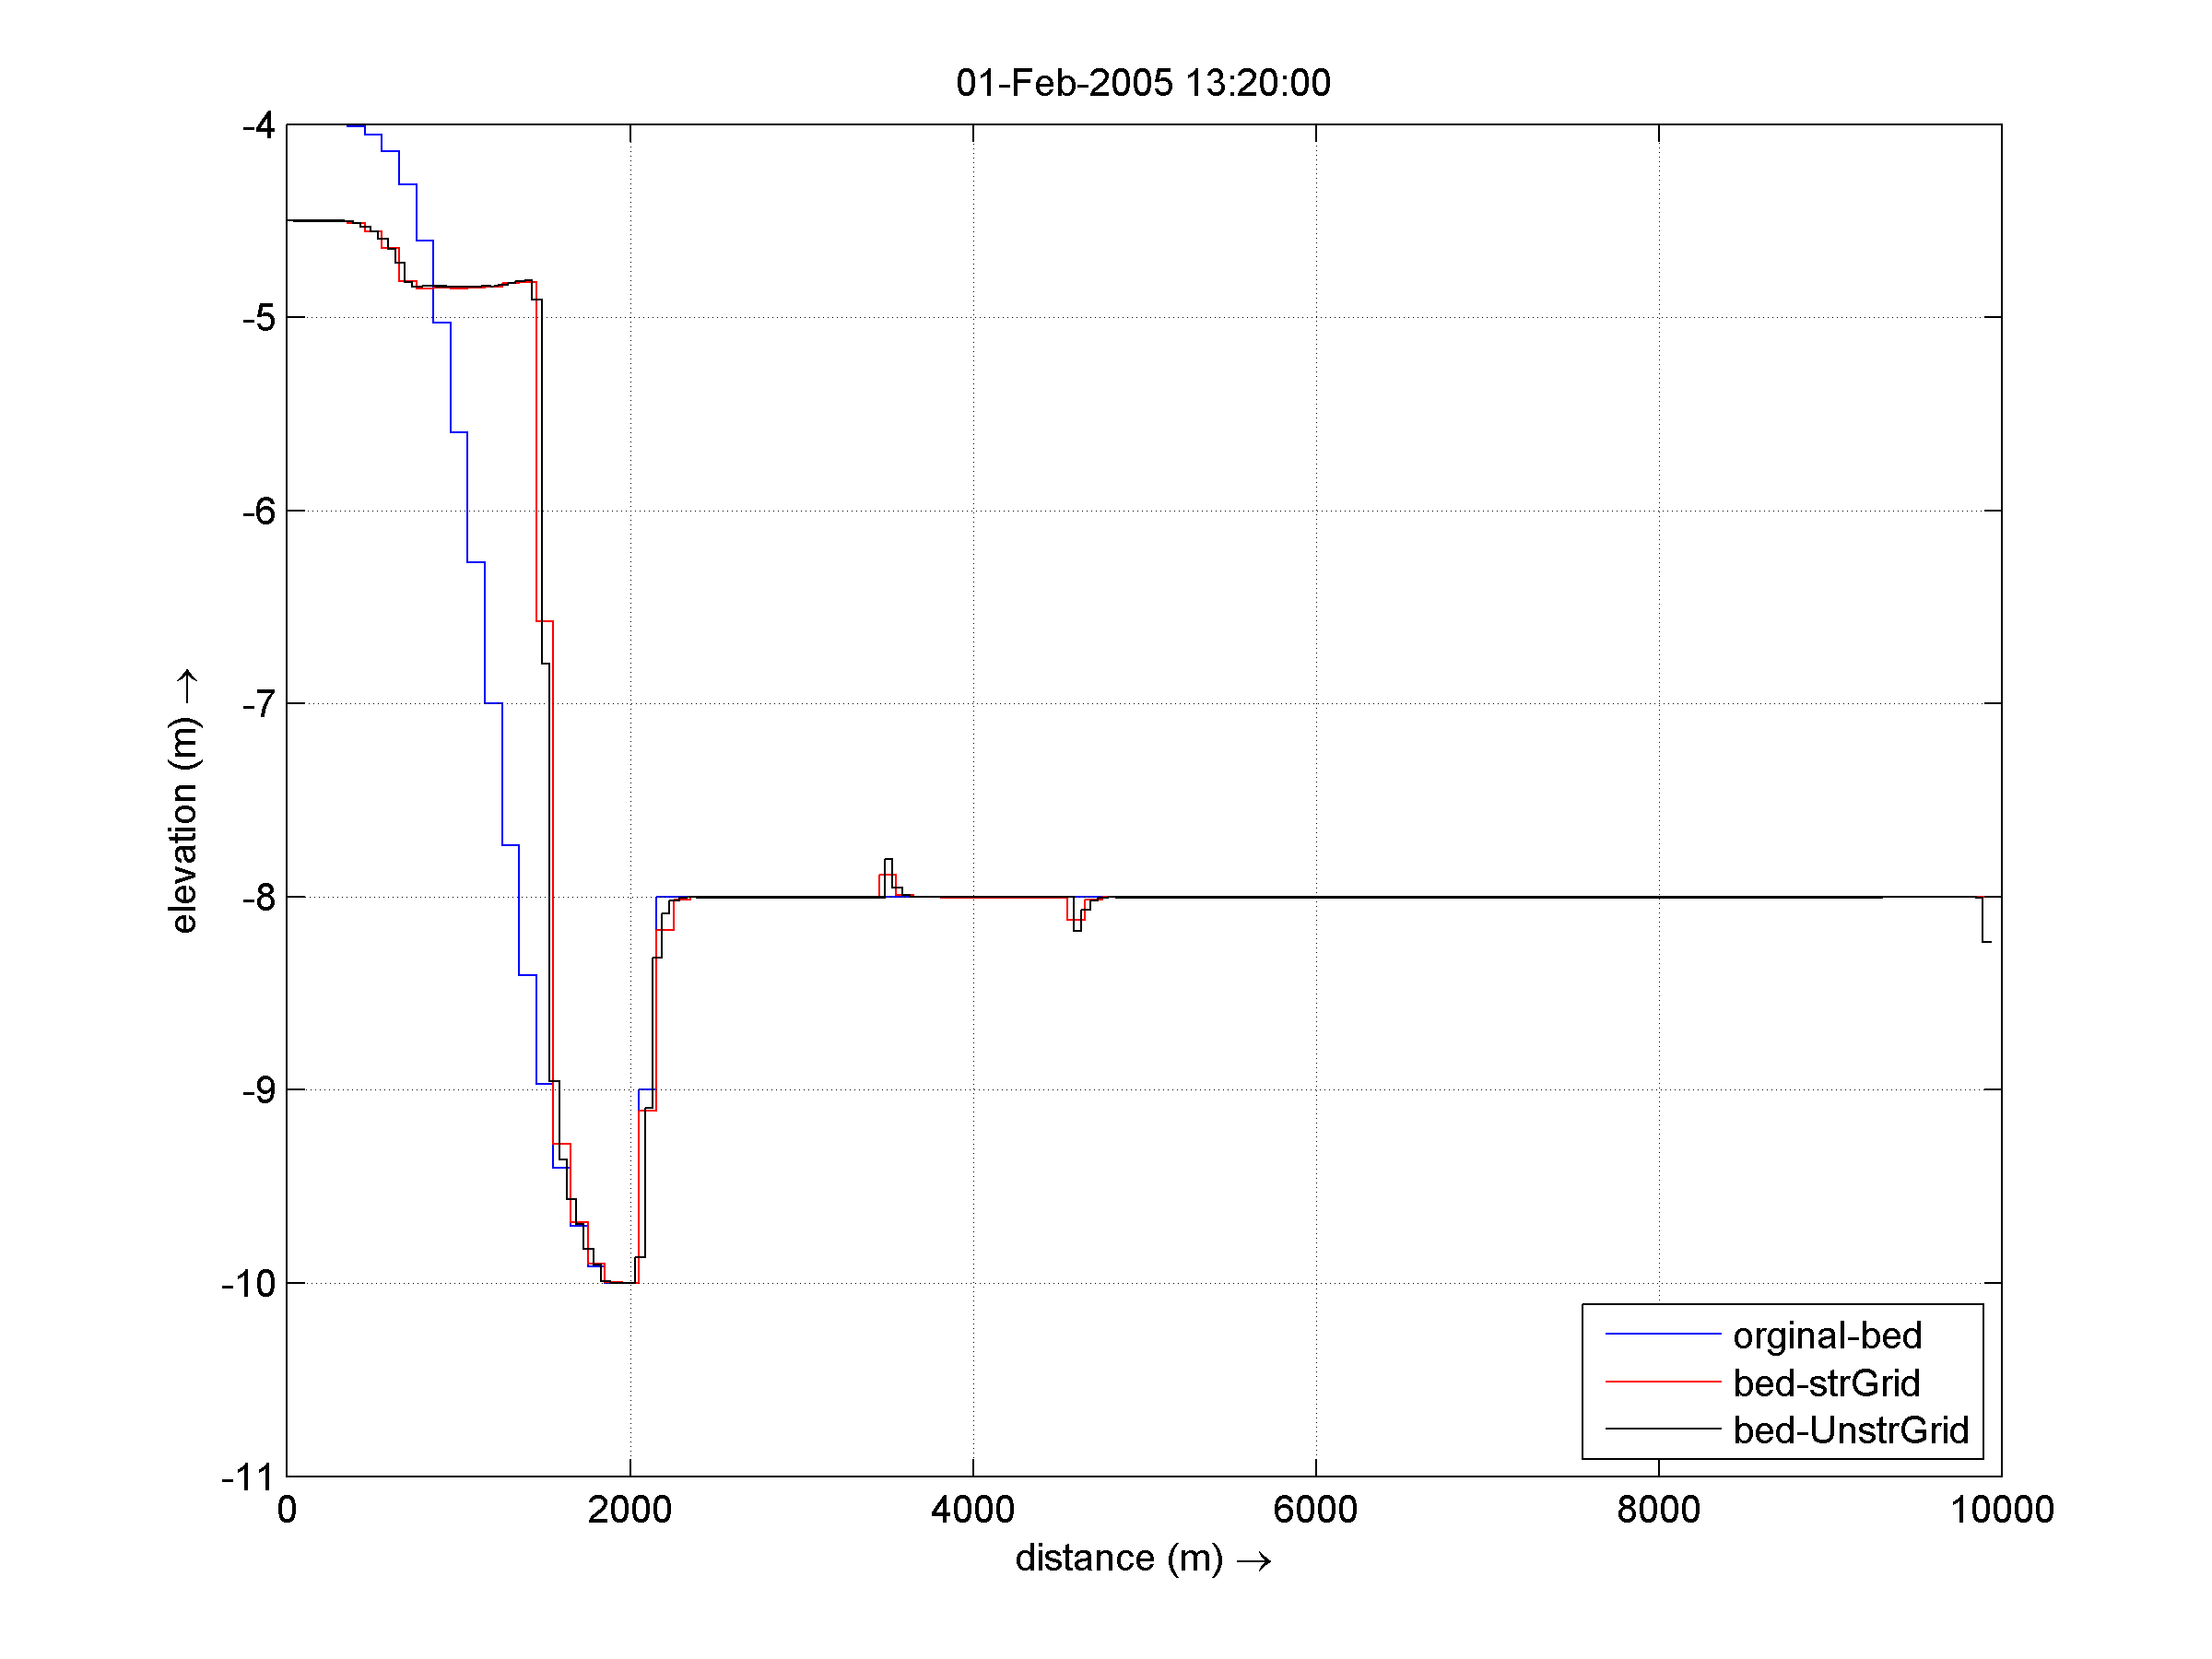
\includegraphics[width=0.7\columnwidth]{figures/C06-bedComparison-55d.png}
	\end{center}\caption{The bed level change along the centerline of the channel after 5.5 days of computation time}
	\label{fig:5.5d}
\end{figure}

\begin{figure}[h!]
	\begin{center}
		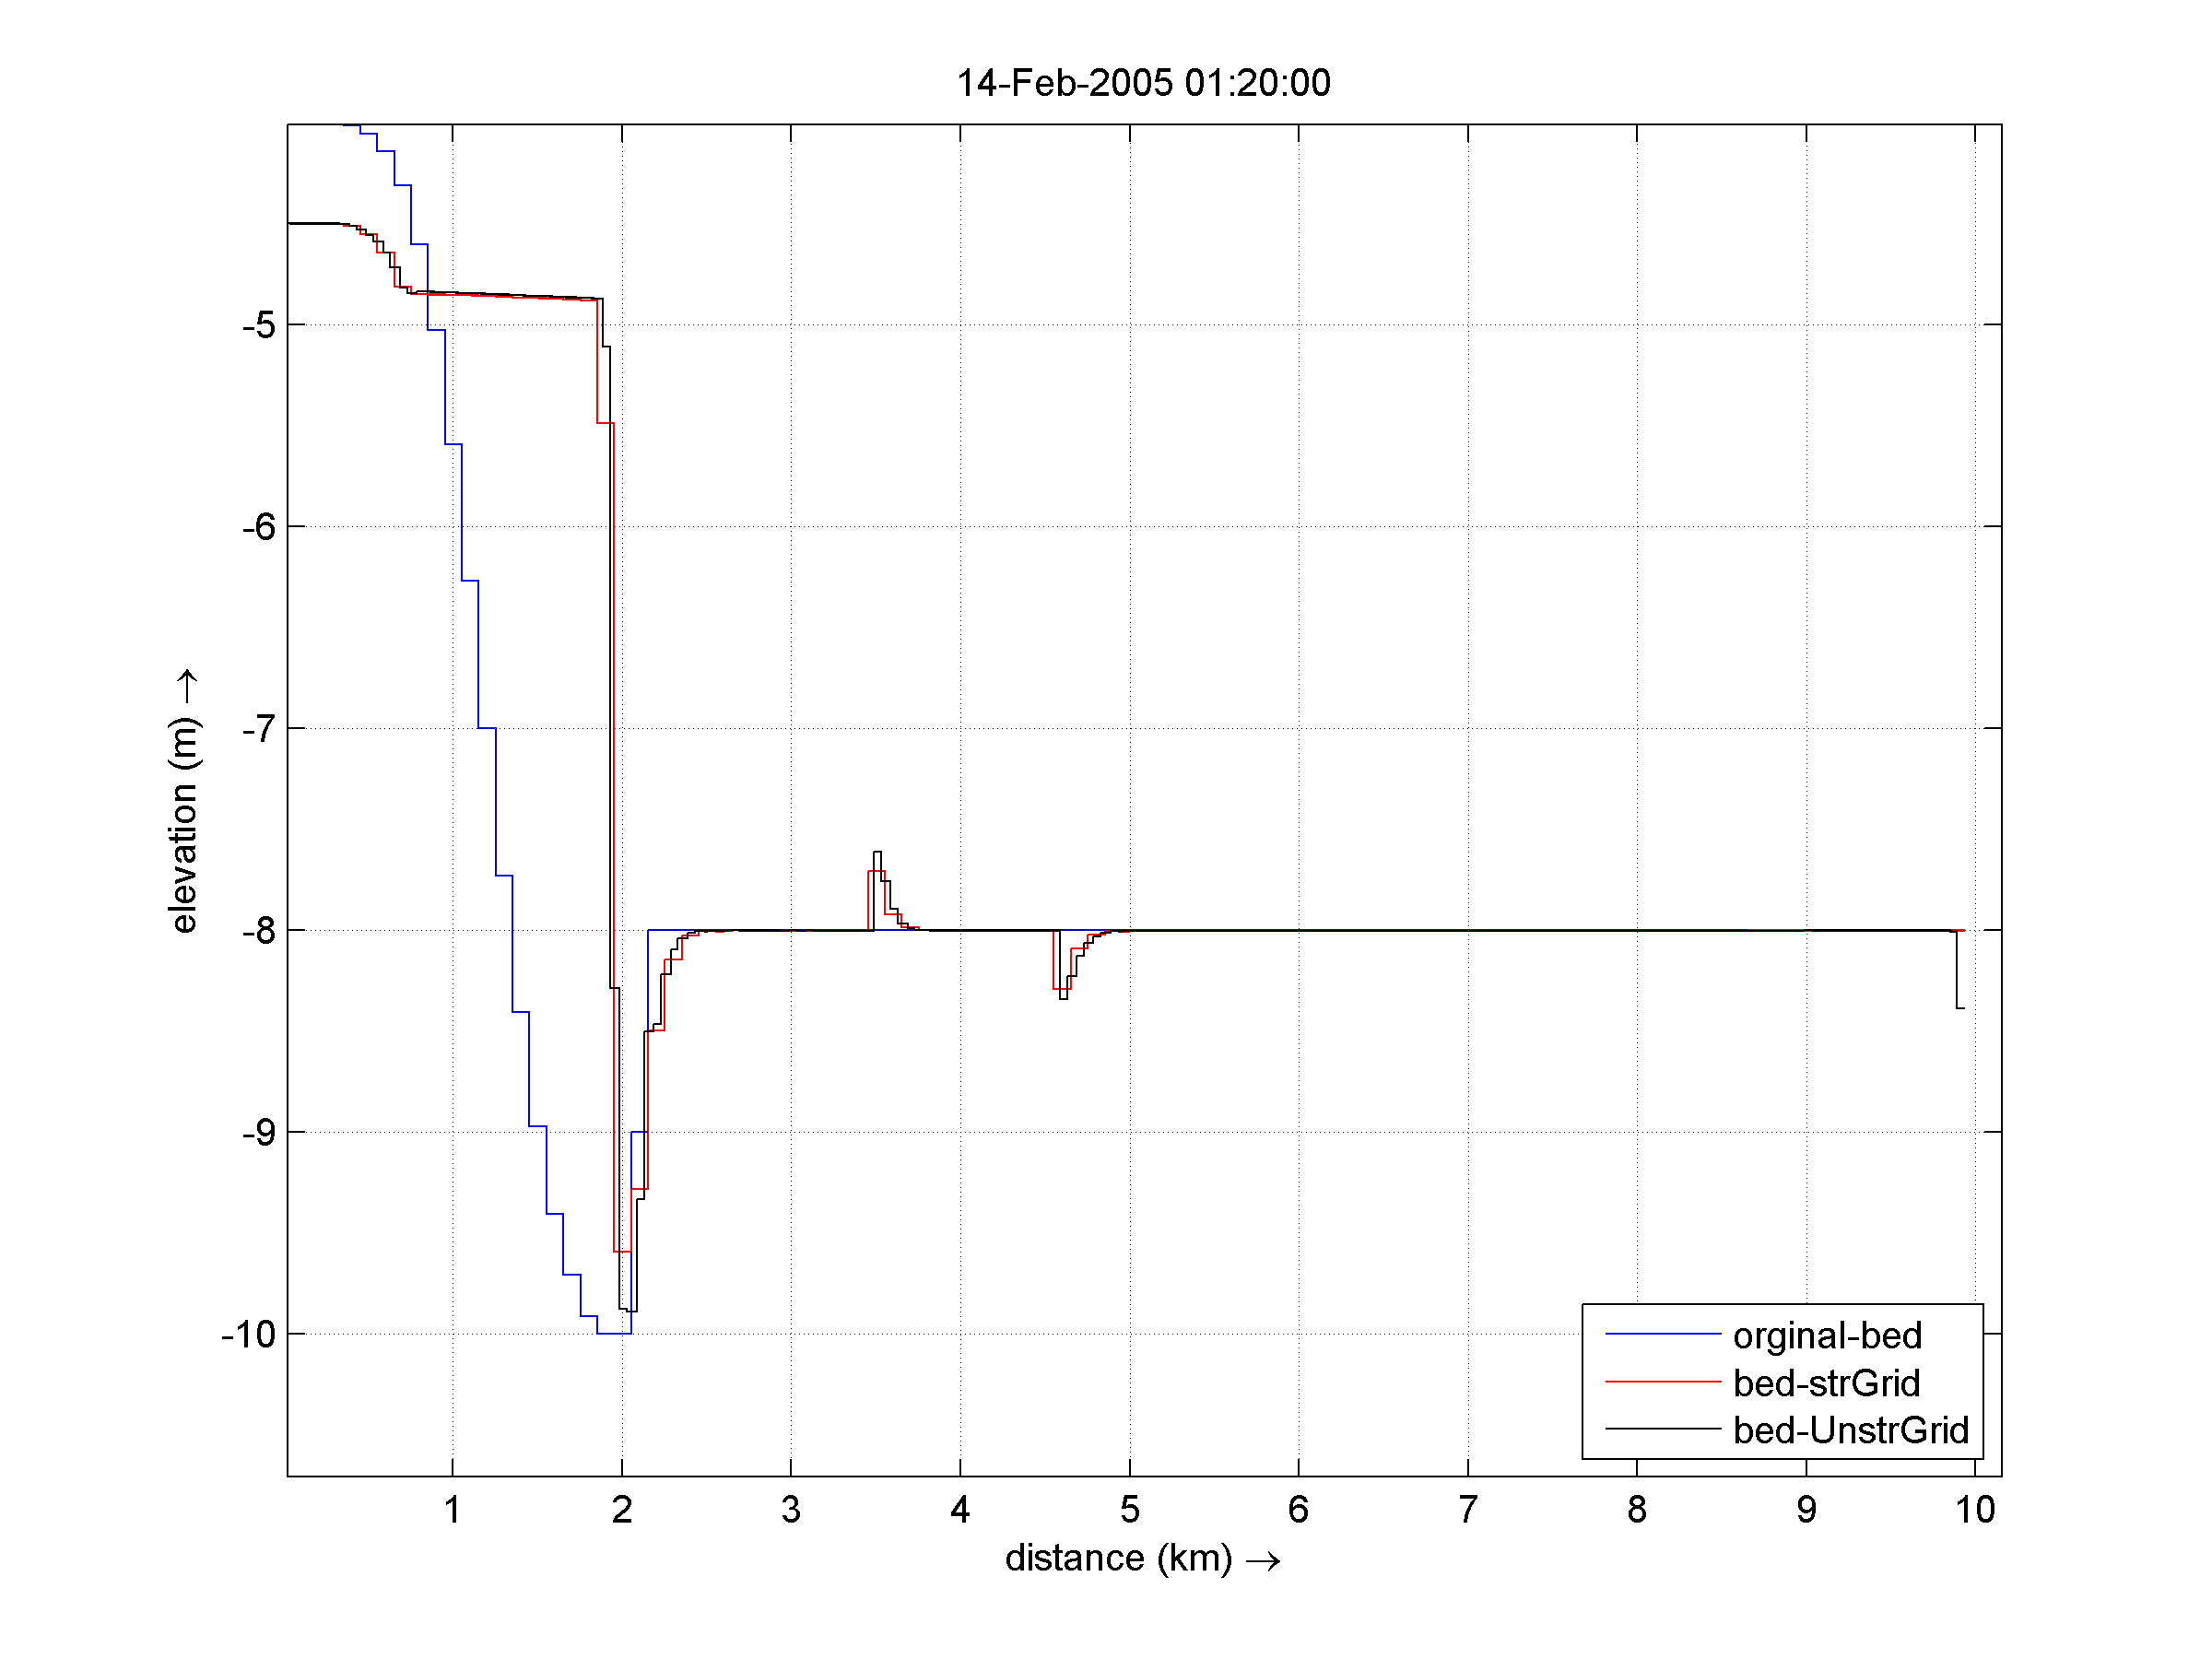
\includegraphics[width=0.7\columnwidth] {figures/C06-bedComparison-18d.png}
	\end{center}\caption{The bed level change along the centerline of the channel after 18 days of computation time}
	\label{fig:18d}
\end{figure}


\paragraph*{Results}

The existing of coarse sand in the middle of the bed composition as shown in figure \ref{fig:ATH}, creates sort of armoring layer in the middle of the channel which creates deposition upstream of this layer and erosion downstream of this layer as shown in figure \ref{fig:5.5d} after 5.5 days, run time, and figure \ref{fig:18d}.

\paragraph*{Conclusion}
The result shows that the variable grain size of uniform sediment work well in FM (Sed-mor)
\paragraph*{Version}
This test has been carried out with the following software versions:
\begin{itemize}
	
	\item[$\bullet$] dflow-fm-x64-1.1.188.47075. 
	
\end{itemize}

%------------------------------------------------------------------------------
%\end{document}
